\documentclass{article}
\usepackage[portuguese]{babel}
\usepackage[letterpaper,top=2cm,bottom=2cm,left=3cm,right=3cm,marginparwidth=1.75cm]{geometry}
\usepackage{amsmath}
\usepackage{graphicx}
\usepackage[colorlinks=true, allcolors=blue]{hyperref}
\usepackage{pgfgantt}

\title{Relatório do EP 1 de MAC0209}
\author{Aurea Maria Emiko Hariki, 9298594\\ Derick William de Moraes Frias, 11207623\\Felipe Pereira Ramos Barboza, 11820322\\Fernando Yang, 13671744\\Marcelo Nascimento dos Santos Junior, 11222012}
\date{14 de maio de 2023}

\begin{document}
\maketitle


\begin{abstract}
Exercício de modelagem com experimentos reais sobre queda livre e pêndulo.
\end{abstract}

\newpage

\tableofcontents

\newpage

\section{Introdução}

Nesta disciplina, estudamos a modelagem de sistemas reais a partir de fenômenos físicos, fórmulas matemáticas e algorítmos. Este exercício programa vai analisar dois fenômenos: Queda livre e Pêndulos. Realizamos experimentos, coletamos dados utilizando o aplicativo Physics Toolbox e analizamos os resultados obtidos.

\section{Objetivos}

Ao simular fenômenos físicos, desenvolver algorítmos e estudar os resultados obtidos, utilizamos as ferramentas e aprendizado obtidos nas aulas e nos materiais auxiliares e gostaríamos que se comportassem de forma similar aos modelos ideais.
\\
Preparamos também um vídeo sobre o desenvolvimento do projeto e os experimentos: \\ \href{https://www.youtube.com/watch?v=qw1PObkObhY}{https://www.youtube.com/watch?v=qw1PObkObhY}.

\section{Cronograma}

Durante as semanas disponíveis para a realização do EP, nosso grupo se organizou sa seguinte forma: a primeira semana foi reservada para formação do grupo e planejamento do cronograma; na segunda semana realizamos e gravamos os experimentos, a partir desse momento começamos o tratamento dos dados e estudo da parte teórica e prática para desenvolver os algorítmos, além disso, também gravamos material auxiliar para o vídeo e começamos a edição. Então, começamos a fazer a modelagem dos fenômenos e o relatório.
\\

\begin{ganttchart}{1}{7}
  \gantttitle{Preparação do EP}{7} \\
  \gantttitlelist{1,...,6}{1} \\
  \ganttbar{Planejamento}{1}{1} \\
  \ganttbar{Experimentos}{2}{2} \\
  \ganttbar{Tratamento de dados}{2}{4} \\
  \ganttlinkedbar{Modelagem}{4}{6} \\
  \ganttlinkedbar{Relatório}{4}{6} \\
  \ganttbar{Vídeo}{2}{6} \\
\end{ganttchart}

\section{Dados e métodos}
\textbf{Materiais:}\\
Corda\\
Celular de 179g\\
Estojo de massa desconsiderada \\
\textbf{Metodologia:}
\begin{itemize}
    \item O celular com o aplicativo Physic ToolBox rodando foi colocado dentro de um estojo. O estojo com o celular dentro foi amarrado a uma corda e a sua outra extremidade foi amarrada a um ponto fixo que deixava o estojo com celular suspenso. Dessa forma, ao realizar os experimentos o celular não era danificado.
    \item Antes de realizar o experimento, balançamos o celular algumas vezes, esperamos alguns segundos e em seguida o soltamos. Ao terminar o experimento, balançamos o celular novamente.
\end{itemize}
\textbf{Dados e modelagem:}\\

O aplicativo utilizado fornece os valores de $\dfrac{F_n}{P}$, onde $F_n$ é a força normal na direção de um dos eixos $x, y$ ou $z$, e $P$ é a força peso do objeto. Portanto, a interpretação adequada para os dados obtidos é que eles representam a aceleração normal exercida sobre o celular, em unidade de $G$.

Os dados de cada experimento foram tratados, de maneira a obter uma coleção de dados boa o sufuciente para estimar os parâmetros desejados. Para isso, foram removidos os dados do acelerômetro antes do início do experimento. Para a queda-livre, foi observado o gráfico do acelerômetro e selecionamos o intervalo de tempo onde ocorreu a queda. Já no experimento do pêndulo, encontramos o início do movimento e arbitramos um fim do experimento comum, que ocorre depois de várias oscilações do pêndulo. \\

Para o experimento da queda-livre, o movimento do corpo foi modelado pela equação diferencial: \begin{equation}\ddot{y} = g - \dfrac{k}{m}\dot{y}^2.\end{equation}
Onde $y$ denota a posição do objeto na vertical, $g$ denota a gravidade, $m$ a massa do objeto e $k$ o coeficiente de atrito. A partir do método de euler e utilizando os dados experimentais, podemos traçar a trajetória da velocidade e da posição do objeto em função do tempo: $$y_{t+1} = y_t + \dot{y}_t\cdot dt $$$$ \dot{y}_{t+1} = \dot{y}_t + \ddot{y}_t \cdot dt.$$
Após obter a aproximação da velocidade experimental, podemos substituí-la na equação (1), e assim obter o coeficiente de atrito $k$: $$k_t = \dfrac{m(\ddot{y}_t - g)}{\dot{y}_t}.$$
O coeficiente $k$ foi estimado tomando a média aritmética dos $k_t$ obtidos. Após a estimação de $k$, foi realizada a sumulação utilizando o método de euler, tomando a equação para a aceleração dada por (1).

No experimento do pêndulo, o movimento do corpo foi modelado pela equação diferencial: \begin{equation} \ddot{\theta} = \dfrac{-g}{L}sin{\theta} - \dfrac{kL^2}{m}\dot{\theta}^2.\end{equation}
Onde $\theta$ denota o ângulo da corda em relação ao eixo vertical e $L$ denota o comprimento da corda. Como o corpo doi lançado na mesma posição da queda-livre, podemos aproveitar o coeficiente de atrito $k$ obtido no experimento anterior, e utilizamos o método de euler para traçar as trajetórias simuladas do movimento pendular.

Para traçar as trajetórias experimentais de $\dot{x}, \dot{y}, x$ e $y$, interpretamos a aceleração normal obtida experimentalmente com o sentido radial, pois a única força exercida sobre o corpo (além do peso) é a tração do fio, que é sempre raidal. O eixo que se alinha à tração, no nosso experimento, é o eixo $y$ do celular. Então, o passo de euler testado foi: $$x_{t+1} = x_t + \dot{x}_t\cdot dt$$ $$y_{t+1} = y_t + \dot{y}_t \cdot dt$$ $$\dot{x}_{t+1} = \dot{x}_t + \left( a_r \dfrac{x_t}{L}\right) dt$$ $$\dot{y}_{t+1} = \dot{y}_t + \left( g - a_r \dfrac{y_t}{L}\right) dt.$$
Onde $a_r$ denota a aceleração radial, obtida experimentalmente.

Entretanto, em nossas tentativas, a aproximação das velocidade e posição do pêndulo em cada instante do tempo não apresentou o comportamento previsto.\\



\subsection{Queda Livre}
\textbf{Metodologia:}
\begin{itemize}
    \item O estojo com o celular dentro foi amarrado a uma corda.
    \item A outra extremidade da corda foi amarrada a uma barra de segurança na ponte da entrada do CCSL.
    \item A altura total da corda esticada era de 3.3m.
    \item O experimento consiste em soltar o celular e deixá-lo em queda livre.
    \item O exeprimento foi repetido 7 vezes.
\end{itemize}

\subsection{Pêndulo}
\textbf{Metodologia:}
\begin{itemize}
    \item O estojo com o celular dentro foi amarrado a uma corda.
    \item A outra extremidade da corda foi amarrada ao galho de um árvore localizada entre a FAUD e o IGc.
    \item A altura total da corda esticada era de 1m.
    \item O celular foi solto a partir de uma altura similar ao do ponto onde a corda foi presa à arvore, criando o movimento de pêndulo.
    \item O experimento foi repetido 5 vezes.
\end{itemize}

\section{Resultados experimentais}
Geramos gráficos de cada experimento e do sinal médio de todas as repetições sobrepostas.


\subsection{Queda Livre}
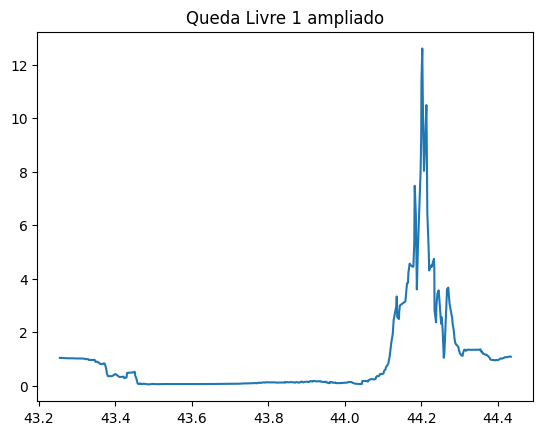
\includegraphics{Q1.png}\\
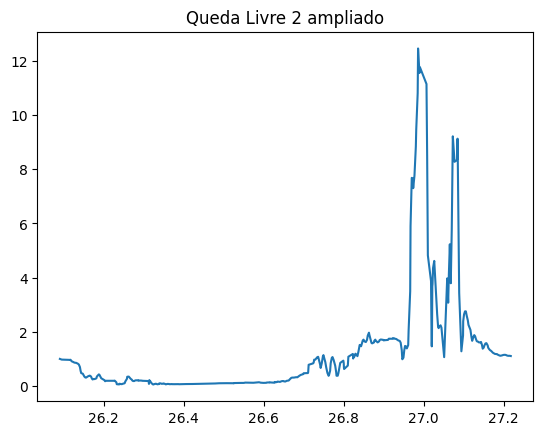
\includegraphics{Q2.png}\\
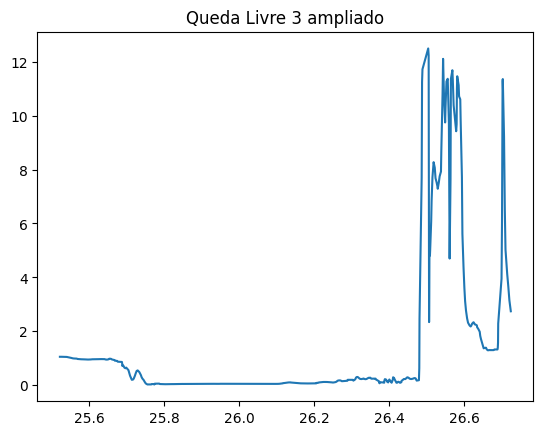
\includegraphics{Q3.png}\\
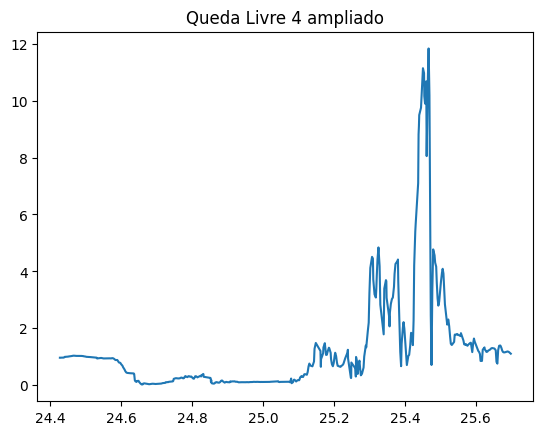
\includegraphics{Q4.png}\\
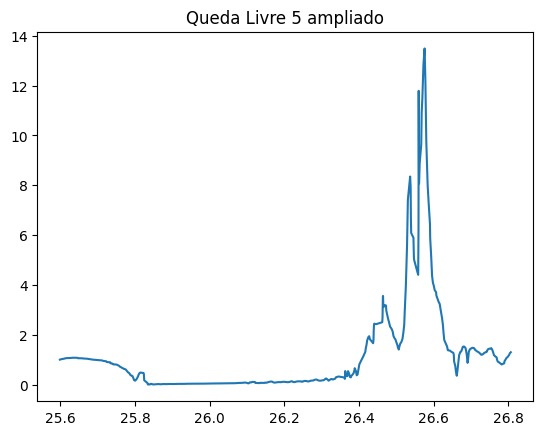
\includegraphics{Q5.png}\\
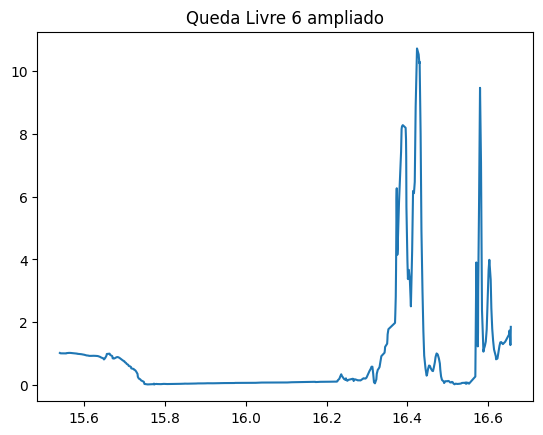
\includegraphics{Q6.png}\\
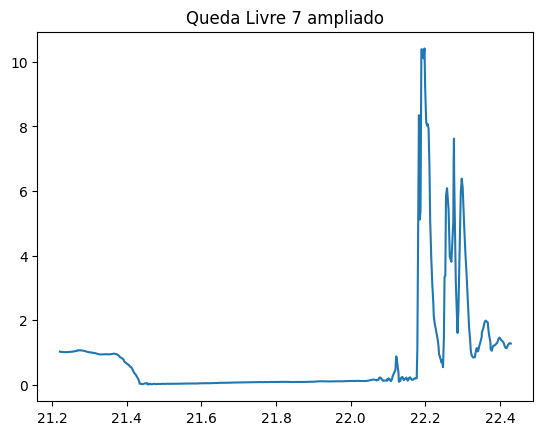
\includegraphics{Q7.png}\\
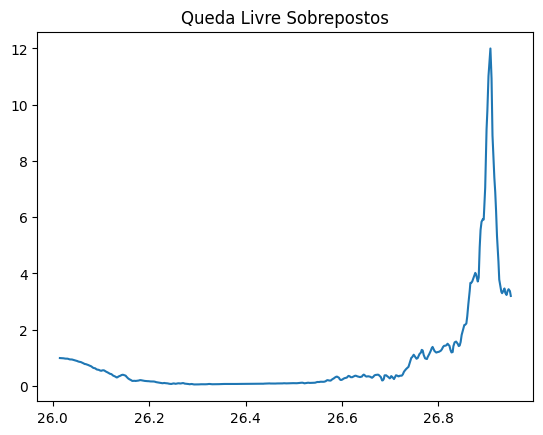
\includegraphics{Q-sobreposto.png}\\

Note que, nos sinais de queda-livre, podemos observar uma inclinação da aceleração normal: Inicialmente é igual a zero, e cresce com a progressão do movimento. Este fenômeno acontece devido à força de atrito do ar, que em nosso modelo, é proporcional ao quadrado da velocidade. Os picos de força, presentes nos finais do experimento, são causados pelo fim abrupto do movimento.

\subsection{Pêndulo}

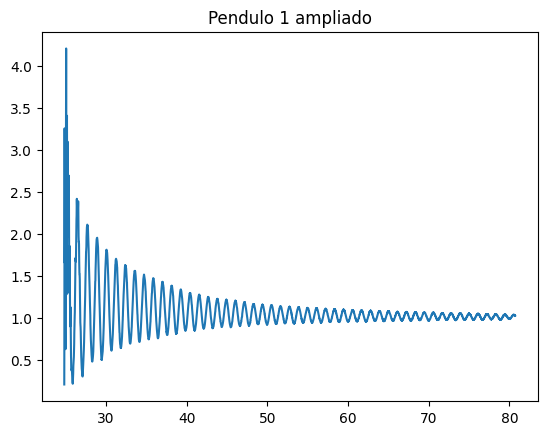
\includegraphics{P1.png}\\
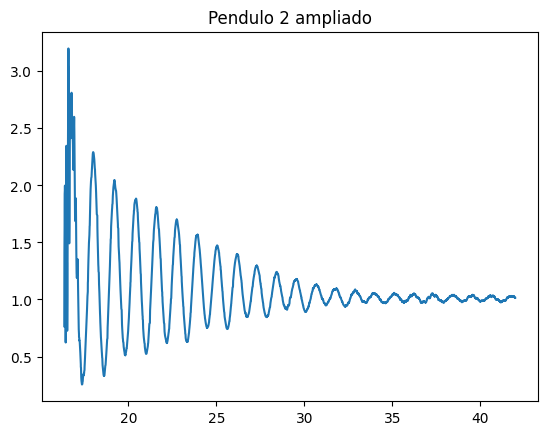
\includegraphics{P2.png}\\
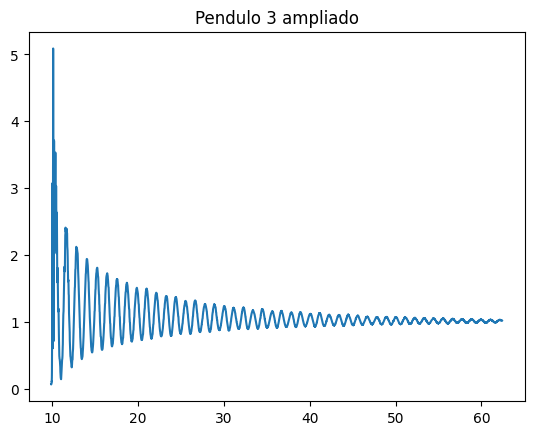
\includegraphics{P3.png}\\
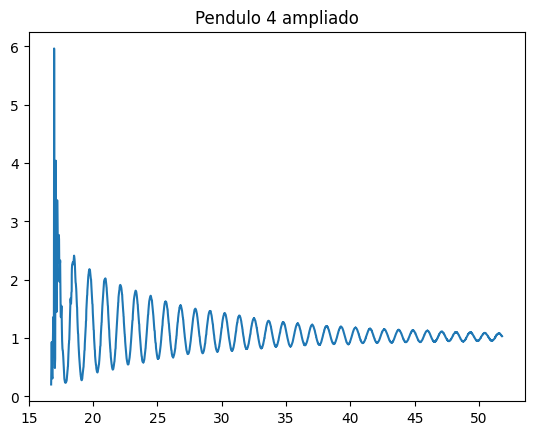
\includegraphics{P4.png}\\
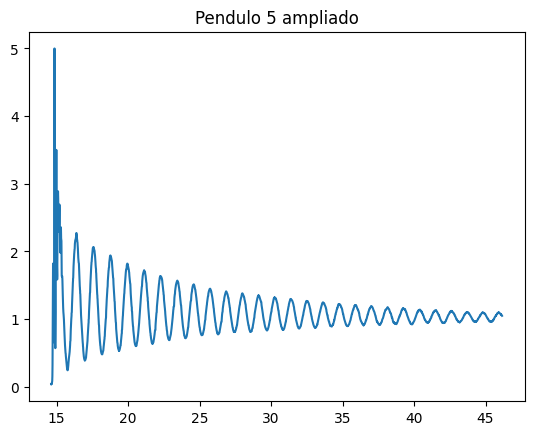
\includegraphics{P5.png}\\
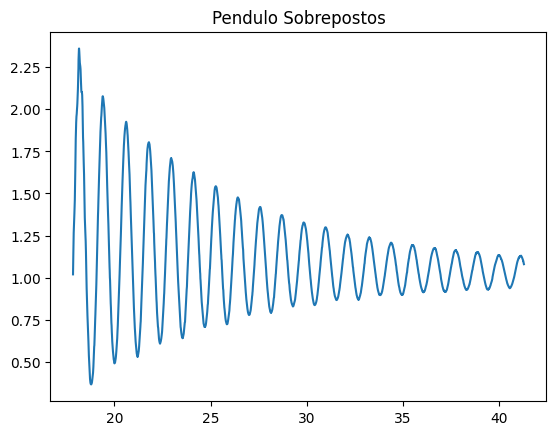
\includegraphics{P-sobreposto.png}\\

Podemos observar que a força normal atinge picos mais altos no início do movimento, e decresce exponencialmente. Os picos são interpretados como os momentos onde a velocidade é máxima no movimento pendular, aproximandamente no ponto mais baixo do movimento, e decrescem com o tempo, devido à armotização da força de atrito do ar. Note que a força medida tende a 1, isto é, no final do experimento, há um equilíbrio entre a força normal (tração no fio) e o peso do objeto.

\section{Conclusão}

Obtivemos simulações satisfatórias para o movimento de queda-livre, onde podemos observar proximidade entre os gráficos dos dados reais e aproximações para velocidade e posição, e a simulação pelo método de euler.\\

Já no experimento de movimento pendular, obtivemos bons resultados para a simulação e os dados gerados pelo aplicativo, porém nossas aproximações para a velocidade e posição em cada instante de tempo não condizem com a realidade. Acreditamos que os erros têm fonte na imprecisão dos dados do experimento, bem como a baixa taxa de convergência do método de euler, que podem ter sido responáveis pela extrapolação das trajetóras traçadas.

\subsection{Queda Livre}

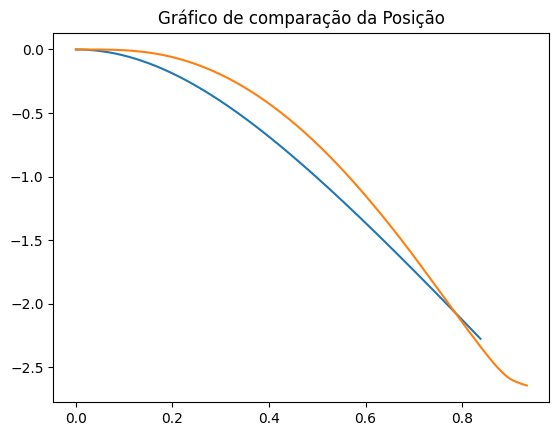
\includegraphics{Q-comparacao-tempo-altura.png}\\
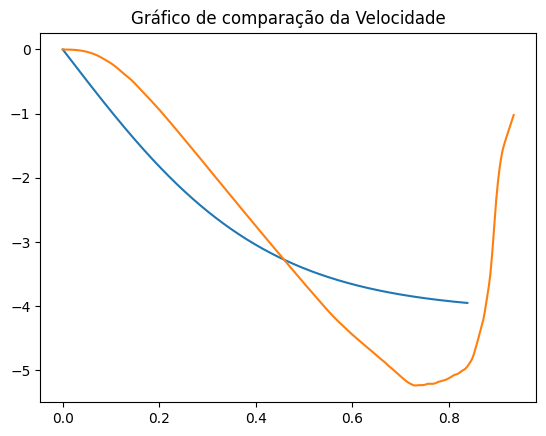
\includegraphics{Q-comparacao-tempo-velocidade.png}\\
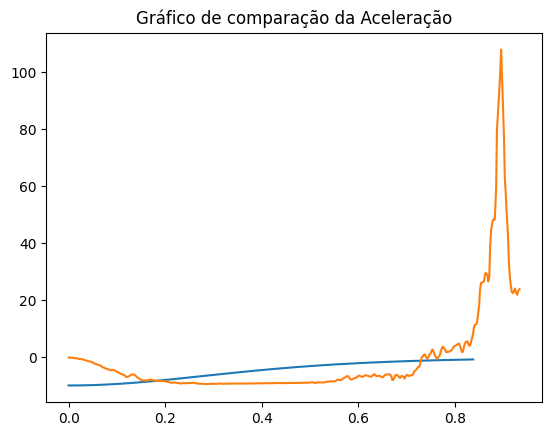
\includegraphics{Q-comparacao-tempo-aceleracao.png}\\

Notamos que os gráficos da simulação e do experimento são similares. No gráfico de comparação de aceleração, perceba que quando a corda é esticada no experimento há um pico na aceleração.

\subsection{Pêndulo}

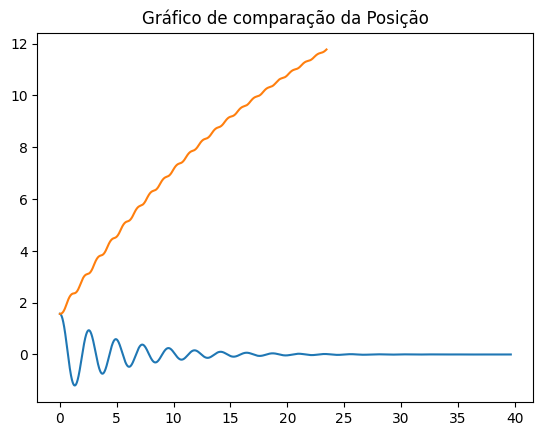
\includegraphics{P-comparacao-posicao.png}\\
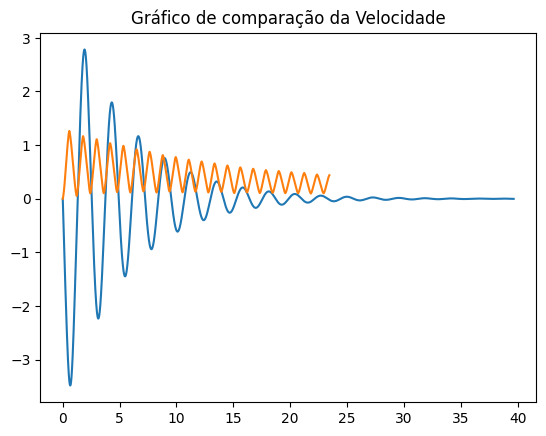
\includegraphics{P-comparacao-velocidade.png}\\
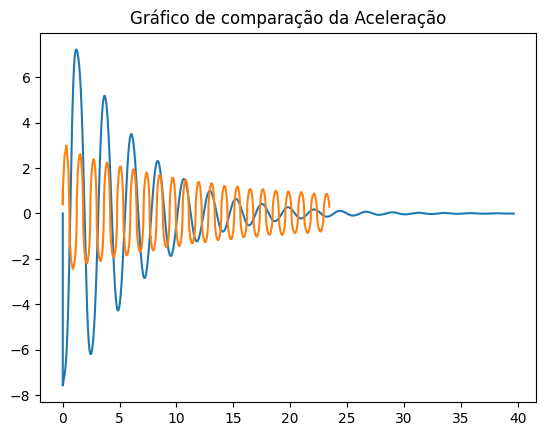
\includegraphics{P-comparacao-aceleracao.png}\\

Encontramos muita dificuldade em encontrar modelos para o pêndulo que descrevesse o fenômeno da forma como o experimento foi realizado.

\end{document}
